\documentclass{../../../fal_assignment}
\graphicspath{ {../../../} }

\usepackage{amsmath}
\usepackage{subcaption}

\hypersetup{
    colorlinks=true, 
    urlcolor=blue,
    linkcolor=
}

\usepackage{listings}
\lstset{
	basicstyle=\ttfamily,
	frame=single,
	showstringspaces=false,
	breaklines=false,
	prebreak={\space\hbox{\textcolor{gray}{$\hookleftarrow$}}}
}
\lstset{
	commentstyle=\ttfamily\textit,
	keywordstyle=\ttfamily\textbf,
	stringstyle=\ttfamily,
	rulecolor=\color{black}
}
\lstset{language=C++}

\title{Worksheet 3: Raycasting}
\author{Kate Bergel}
\module{COMP270}
\version{1.1}

\begin{document}

\maketitle

\section*{Introduction}

In this worksheet you will use 3D vectors and matrices to complete the implementation of a basic ray caster and create an effect to add depth.

Begin by \textbf{forking} the following BitBucket repository:

\begin{center}
	\url{https://gamesgit.falmouth.ac.uk/projects/COMP270/repos/comp270-worksheet-3}
\end{center}

\textbf{Complete} the \textbf{FOUR} tasks described below, remembering to \textbf{commit} your work regularly.
To submit your work, open a \textbf{pull request} from your forked repository to the original repository.

\textbf{Note}: The tasks below can be completed by filling in the relevant functions marked in \texttt{Camera.cpp} and \texttt{Object.cpp}, however you are welcome (and encouraged) to add appropriate helper methods and member data to relevant classes, especially for Task 4. It should not be necessary to deviate from the main program structure; if you do decide to do so, your reasons should be stated in code comments and/or git commit messages.

Aside from the first task, which must be completed in order to actually see anything, the implementations do not depend on one another and may be attempted in any order.

\section*{Background}

\begin{figure}[ht]
	\begin{center}
		\begin{subfigure}[b]{0.45\linewidth}
			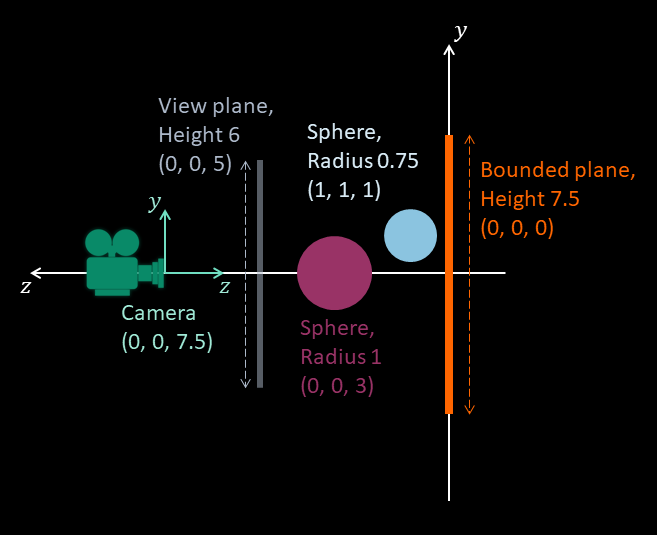
\includegraphics[width=\linewidth]{scene_side}
			\caption{Side view}
		\end{subfigure}
		\begin{subfigure}[b]{0.45\linewidth}
			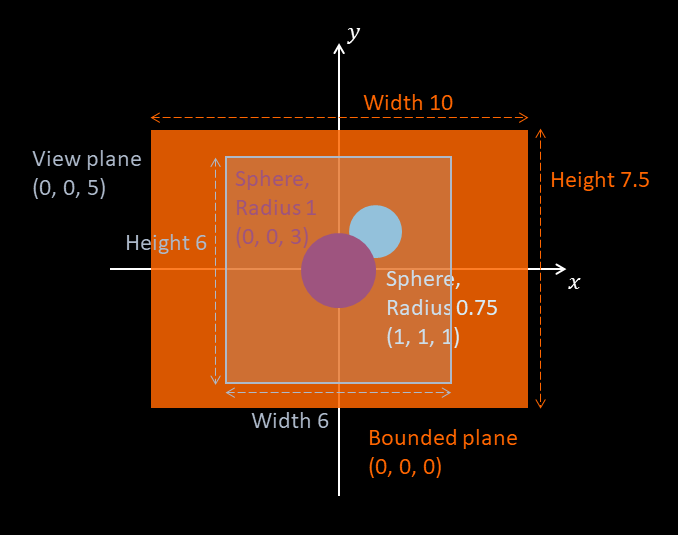
\includegraphics[width=\linewidth]{scene_camera_view}
			\caption{Camera view}
		\end{subfigure}
	\end{center}
	\caption{A diagram of the scene setup with world-space coordinates and dimensions of the objects.}
	\label{fig:scene}
\end{figure}

The provided skeleton project implements a basic raycasting camera setup, as shown in Figure~\ref{fig:scene}.
Some objects - two spheres and a plane - are already in the scene, though they cannot be seen to start with. The camera is initially at the point (0, 0, 7.5) in world space, facing along the negative $z$-axis, with its $x$- and $y$-axes aligned with the world coordinates so that they form a \textbf{left-handed} coordinate space, as opposed to the \textbf{right-handed} one of the world.

The camera can be moved in a limited fashion, in directions along the \textbf{world coordinate axes}, with the following key presses:

\begin{itemize}
	\item \lstinline{a}: translates the camera in the negative $x$ direction ("left")
	\item \lstinline{d}: translates the camera in the positive $x$ direction ("right")
	\item \lstinline{s}: translates the camera in the negative $y$ direction ("down")
	\item \lstinline{w}: translates the camera in the positive $y$ direction ("up")
	\item \lstinline{q}:  translates the camera in the negative $z$ direction (towards the objects)
	\item \lstinline{e}:  translates the camera in the positive $z$ direction (away from the objects)
\end{itemize}

In addition, the camera can be "zoomed" in/out by pressing the up/down arrow keys, which moves the view plane away from/towards the camera.

\textbf{Additional settings}: If you need to adjust the colours of the objects to see them more clearly, you can do so in \lstinline{Application::setupScene()}.

\section*{Task 1: let there be light}
\begin{marginquote}
``Happiness can be found, even in the darkest of times, if one only remembers to turn on the light."
\par --- Albus Dumbledore
\end{marginquote}
The camera creates a picture by choosing a colour for each 'pixel' of the view plane based on which object is visible through the pixel from the camera's position. The visibility test is carried out in \lstinline{Camera::updateScreenBuffer} by finding which objects are encountered by 'rays' sent from the camera through the centre of each pixel.

The number and directions of the rays will be determined by the view plane properties stored in the \lstinline{Camera::m_viewPlane} struct, which can be accessed from within \lstinline{Camera} methods as e.g. \lstinline{m_viewPlane.distance}. \textbf{Note} that the view plane \lstinline{distance} is measured along the \textbf{camera's viewing direction}, i.e. the positive $z$ direction in camera space starting from the camera, so that the view plane initially has coordinates (0, 0, 2.5) in camera space and (0, 0, 5) in world space.

The view plane is divided into a grid of 'pixels' with the resolution in each direction giving the number of pixels in that direction as shown in Figure~\ref{fig:pixels}, which also illustrates the measurement of the distance from the camera to the view plane and the pixel indexing.

\begin{figure}[ht]
	\begin{center}
		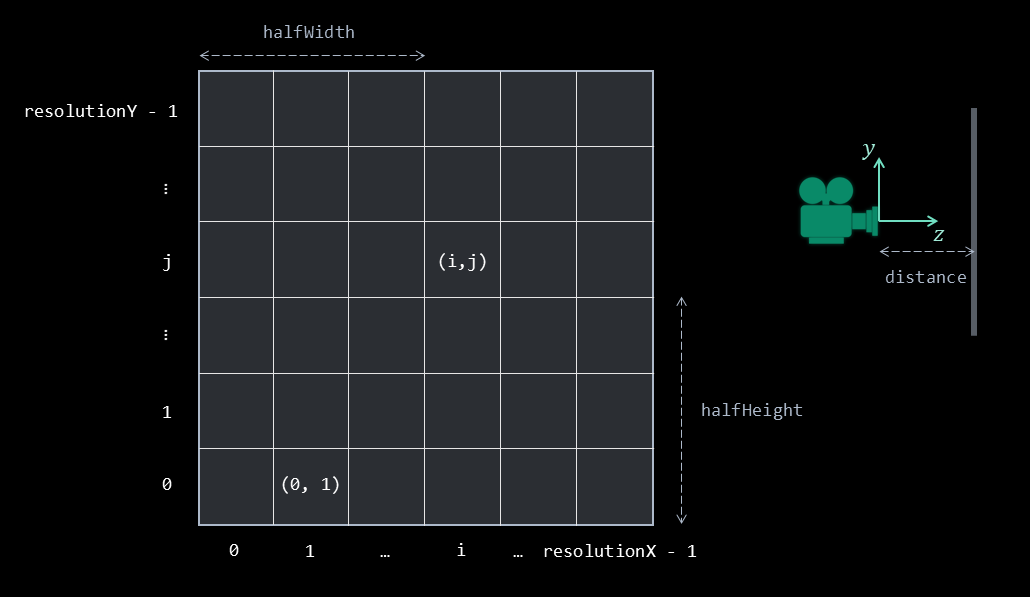
\includegraphics[width=0.5\linewidth]{pixel_grid}
	\end{center}
	\caption{View plane dimensions and positioning}
	\label{fig:pixels}
\end{figure}

Complete the following two steps in \texttt{Camera.cpp} to determine the direction of the rays through the view plane:

\begin{enumerate}[label=(\alph*)]
	\item \textbf{Add the calculations} in \lstinline{Camera::init()} for finding the width and height of each pixel (in camera-space units), storing the results in \lstinline{m_pixelWidth} and \lstinline{m_pixelHeight} (these values are used in various functions).
	\item \textbf{Implement} \lstinline{Camera::getRayDirectionThroughPixel()} to return the \textbf{normalised direction in camera space} of the ray starting at the camera's position and passing through the \textbf{centre} of pixel in the view plane with grid index \lstinline{(i, j)}. Note that the grid indices should correspond to the coordinate frame of the scene/camera, where the $y$ axis points upwards, \textbf{not} the SDL screen coordinates.
\end{enumerate}

Once you've generated the rays, you should be able to see the spheres as in Figure~\ref{fig:spheres}. You'll notice that the image appears fairly blocky, as a relatively low resolution has been set to keep processing times reasonable; you can reduce the blockiness by increasing the values of \lstinline{Camera::m_viewPlane.resolutionX} and \lstinline{Camera::m_viewPlane.resolutionY}.

\begin{figure}[ht]
	\begin{center}
		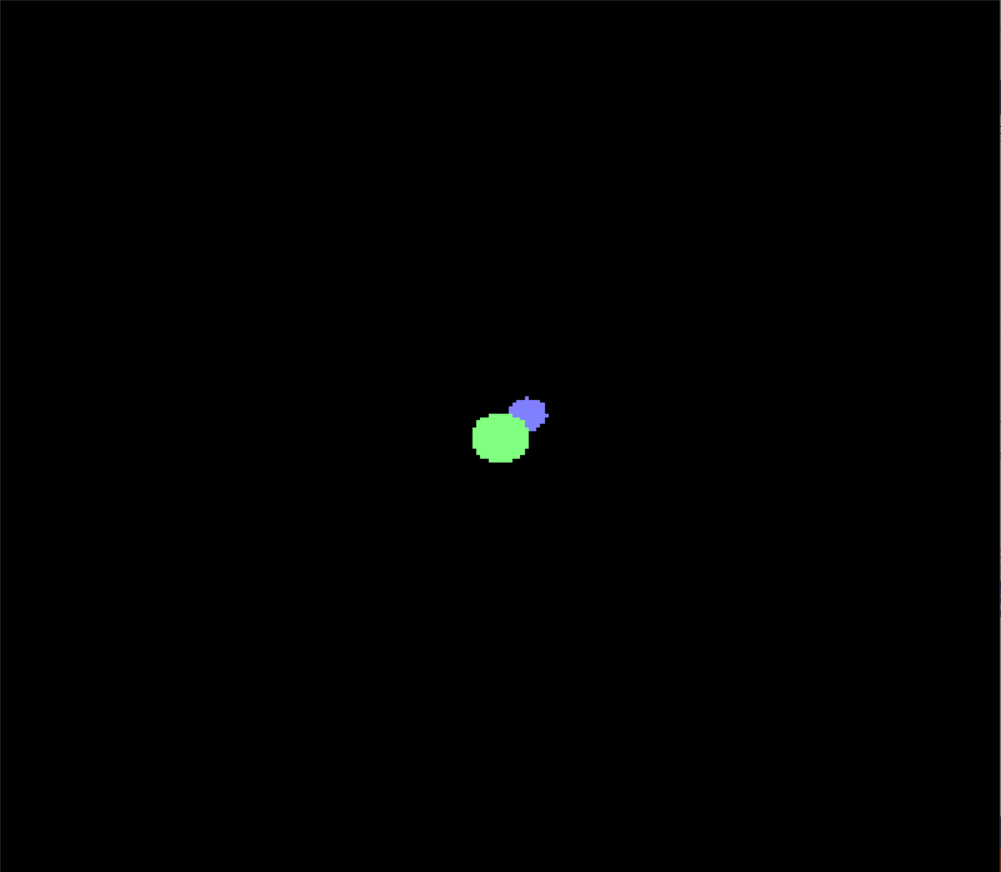
\includegraphics[width=0.25\linewidth]{spheres}
	\end{center}
	\caption{Scene view with ray generation.}
	\label{fig:spheres}
\end{figure}

\section*{Task 2: in plane sight}

There is still one object in the scene that can't be seen yet, because the test to determine whether a ray intersects it is missing. The object is a rectangular plane, which is defined by its normal \lstinline{m_normal} and (optional) dimensions \lstinline{m_halfWidth} and \lstinline{m_halfHeight} that give the distance of the edges from the world-space centre point (\lstinline{m_centre}) along perpendicular vectors \lstinline{m_widthDirection} and \lstinline{m_heightDirection} as shown in Figure~\ref{fig:plane_dimensions}. If either of the half-width or half-height of the plane is zero, the plane is assumed to be infinite.

\begin{figure}[ht]
	\begin{center}
		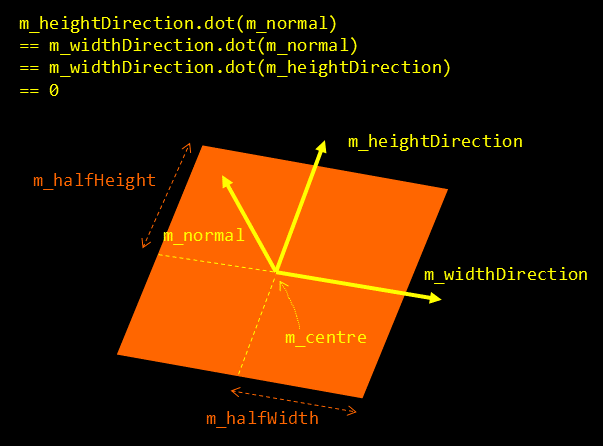
\includegraphics[width=0.5\linewidth]{plane_dimensions}
	\end{center}
	\caption{Properties of a rectangular plane.}
	\label{fig:plane_dimensions}
\end{figure}

\textbf{Implement} \lstinline{Plane::getIntersection()} (in \texttt{Object.cpp}) to return \lstinline{true} if the ray intersects the plane \textbf{within the bounds of its width and height}, and \textbf{set} the parameter \lstinline{distToFirstIntersection} to be the distance along the ray from its source that the intersection occurs (i.e. the parameter $t$ in the equations). Following this, your scene should look like Figure~\ref{fig:plane}.

\begin{figure}[ht]
	\begin{center}
		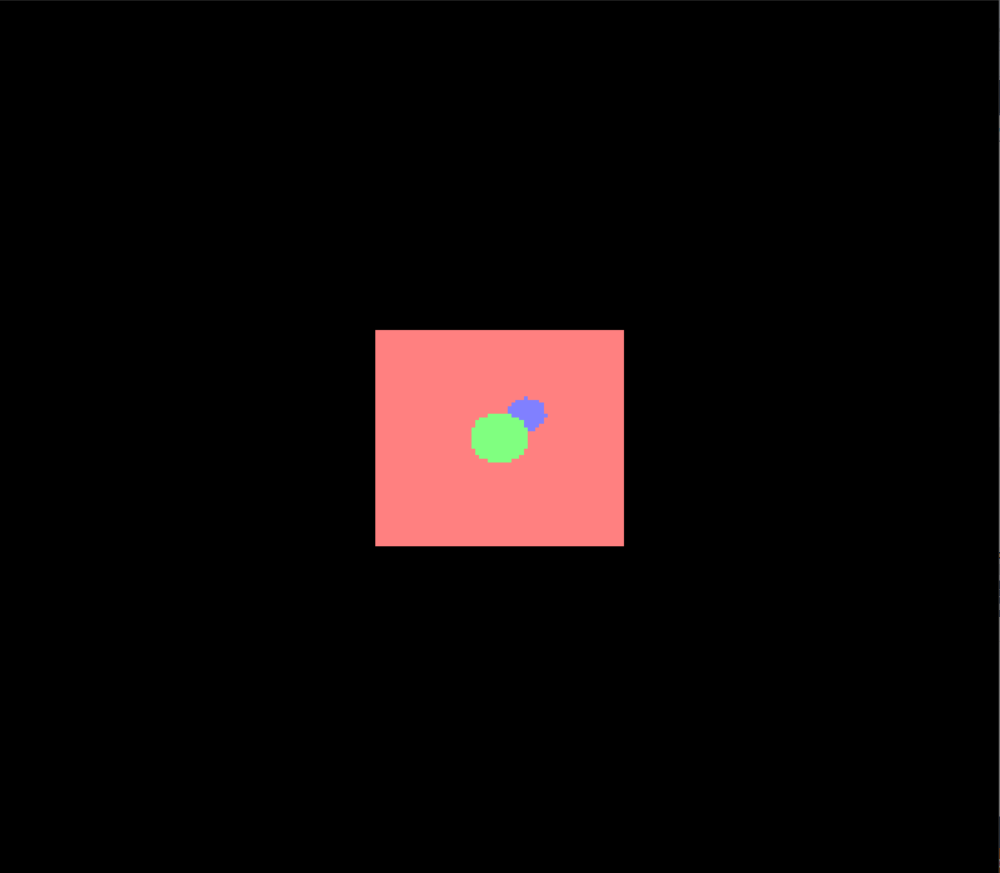
\includegraphics[width=0.25\linewidth]{plane}
	\end{center}
	\caption{Scene view with plane intersection.}
	\label{fig:plane}
\end{figure}

\textbf{Test} that your code works for a variety of plane orientations, not just ones that are aligned with the camera, by changing the plane normal and 'up' directions passed to the plane constructor in \lstinline{Application::setupScene()} - for example, to add a plane with \lstinline{m_normal} = <0.5, 0.5, 1.0> and \lstinline{m_heightDirection} (or \lstinline{up}) = <-0.5, 1.0,-0.25>, you would run the following code, to create a scene that looks like Figure~\ref{fig:tilted_plane}:

\lstinline{m_objects.push_back(new Plane(Point3D(),}\\
\hspace*{30mm}\lstinline{Vector3D(0.5f, 0.5f, 1.0f),}\\
\hspace*{30mm}\lstinline{Vector3D(-0.5f, 1.0f, -0.25f),}\\
\hspace*{30mm}\lstinline{10.0f, 7.5f));}

\begin{figure}[ht]
	\begin{center}
		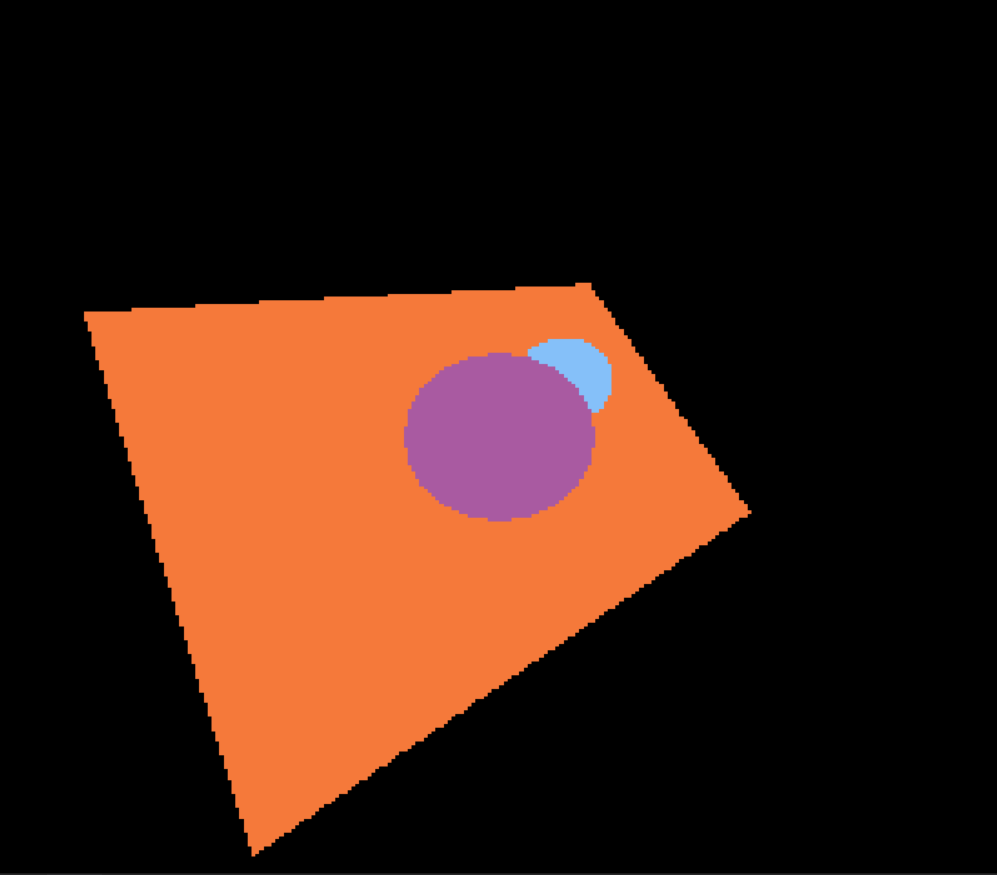
\includegraphics[width=0.25\linewidth]{tilted_plane}
	\end{center}
	\caption{Scene view with tilted plane.}
	\label{fig:tilted_plane}
\end{figure}

\section*{Task 3: spinning around}

Now you can see things, but only in a limited way, as the camera direction is fixed: although holding \lstinline{shift} down when pressing the camera control keys modifies the values in \lstinline{Camera::m_rotation}, these values are not used when determining the scene layout relative to the camera.

\textbf{Modify} \lstinline{Camera::updateWorldTransform()} to compute the \textbf{full transform matrix} of the camera in world space, which is also the matrix that will transform the objects from camera space to world space. The result should be stored in \lstinline{m_cameraToWorldTransform}; you can access the element of a \lstinline{Matrix3D} at row \lstinline{r} and column \lstinline{c} using the \lstinline{()} operator for both get and set:

\hspace*{10mm}\lstinline{// set the value of the matrix at row r, column c}\\
\hspace*{10mm}\lstinline{m_cameraToWorldTransform(r, c) = value;}\\
\hspace*{10mm}\lstinline{// get the value of the matrix at row r, column c}\\
\hspace*{10mm}\lstinline{value = m_cameraToWorldTransform(r, c);}
\begin{marginquote}
``Unfortunately, no-one can be told what the Matrix is. You have to see it for yourself."
\par --- Morpheus
\end{marginquote}

\textbf{Note} that there are various ways in which you can perform the rotation, which may be relative to the camera (as a first person player view) or around the world origin/other point of interest (as in a modelling tool such as Maya). In addition, there are multiple ways to interpret Euler angles, resulting in several possible calculations for converting them into a matrix; any solution is acceptable, provided it allows the scene to be viewed from different angles whilst preserving the relative positions and dimensions of the objects. It is highly likely that you will want to modify the key mappings in \lstinline{Application::processEvent()} to match your particular choice of rotation setup. Also, \textbf{remember} to include the translations and conversion from right- to left-handed coordinates.

With rotations in place, you should be able to view the scene from more interesting angles, such as in Figure~\ref{fig:rotate}.

\begin{figure}[ht]
	\begin{center}
		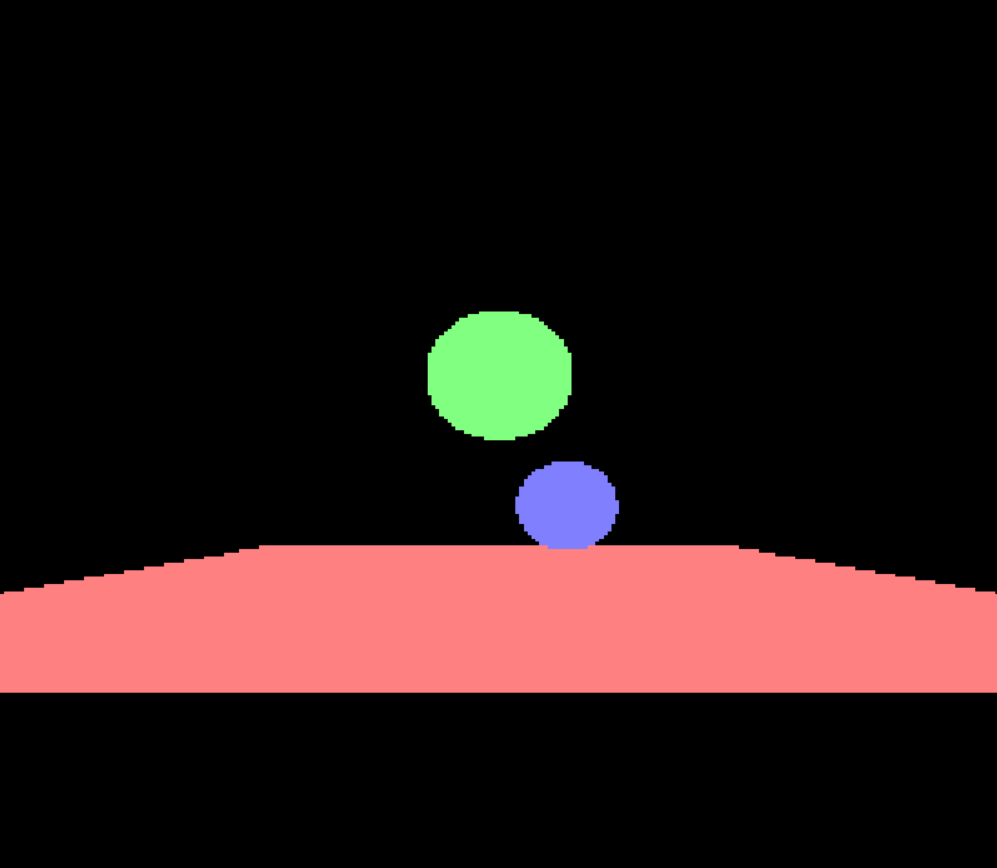
\includegraphics[width=0.25\linewidth]{rotate}
	\end{center}
	\caption{Scene view from a different angle.}
	\label{fig:rotate}
\end{figure}

\section*{Task 4: round things that look round}

So far, everything is looking rather flat because we're setting all the pixels to the same colour, regardless of how far away the object is or how the intersected surface is oriented, when in reality there would be shadows, reflections and a number of other effects adding depth to the scene. There is a variety of methods to simulate these effects, known as \href{https://www.scratchapixel.com/lessons/3d-basic-rendering/introduction-to-shading}{shading}, with different levels of complexity, including
\begin{itemize}
	\item applying a '\href{https://en.wikipedia.org/wiki/Distance_fog}{distance fog}'-like effect to modulate the colour intensity depending on the distance from the camera.
	\item modifying the colour based on the surface orientation (given by the \href{https://mathworld.wolfram.com/NormalVector.html}{surface normal}).
	\item using \href{https://www.scratchapixel.com/lessons/3d-basic-rendering/introduction-to-ray-tracing}{ray tracing} to simulate reflecting the rays from the object's surface and create shadows by testing whether those rays intersect another object before reaching a \href{https://www.scratchapixel.com/lessons/3d-basic-rendering/introduction-to-shading/shading-lights}{light source}.
	\item applying a standard shading technique, such as \href{https://www.scratchapixel.com/lessons/3d-basic-rendering/phong-shader-BRDF}{Phong} or \href{https://www.scratchapixel.com/lessons/3d-basic-rendering/introduction-to-shading/diffuse-lambertian-shading}{Lambert} shading, to approximate lighting effects more efficiently than with ray tracing.
\end{itemize}

\textbf{Choose} (or \textbf{invent}) and \textbf{implement} a method for giving the scene a "more 3D" look - points will be awarded for creativity as well as adherence to existing techniques, and for interesting as well as realistic effects!

The colour for a pixel is currently computed in \lstinline{Camera::getColourAtPixel()}, which is supplied with the pixel indices as input arguments, and has access to the closest object to the pixel and the distance to the point of intersection via the \lstinline{ObjectInfo} stored in \lstinline{m_pixelBuf} - you can also retrieve the direction of the ray that intersects the object by calling \lstinline{getRayDirectionThroughPixel(i, j)}, plus all the other members of the \lstinline{Camera} class are of course available. For simple techniques, this may be enough, however you could also extend the functionality by saving additional information from the intersection test (see comments in the code for how).

\rubrichead{All submissions and assessment criteria for this assignment are individual. To \textbf{pass} this assignment (achieve 40\% or more), you must submit a reasonable attempt at the worksheet by the formative deadline stated on LearningSpace.}
\begin{markingrubric}

	\firstcriterion{Basic competency threshold}{30\%}
		\grade\fail	A reasonable attempt at the worksheet was not submitted by the formative deadline.
		\par Evidence of breach of academic integrity.
		
    \criterion{PROCESS:\\Functional coherence}{40\%}
        \grade\fail None of the tasks have been attempted.
		\grade Task 1 has been attempted and partially completed.
		\grade Task 1 has been successfully completed.
		\grade Two tasks (including task 1) have been successfully completed.
		\grade Three tasks (including task 1) have been successfully completed.
		\grade All four tasks have been successfully completed.

    \criterion{PROCESS:\\Maintainability}{30\%}
        \grade \fail The code is only sporadically commented, if at all, or comments are unclear.
            \par Few identifier names are clear or inappropriate.
            \par Code formatting hinders readability.
        \grade The code is well commented.
            \par Some identifier names are descriptive and appropriate.
            \par An attempt has been made to adhere to a consistent formatting style.
             \par There is little obvious duplication of code or of literal values.           
        \grade The code is reasonably well commented.
            \par Most identifier names are descriptive and appropriate.
            \par Most code adheres to a sensible formatting style.
             \par There is almost no obvious duplication of code or of literal values.   
        \grade The code is reasonably well commented, with appropriate high-level documentation.
            \par Almost all identifier names are descriptive and appropriate.
            \par Almost all code adheres to a sensible formatting style.
             \par There is no obvious duplication of code or of literal values. Some literal values can be easily ``tinkered''. 
        \grade The code is very well commented, with comprehensive appropriate high-level documentation.
            \par All identifier names are descriptive and appropriate.
            \par All code adheres to a sensible formatting style.
             \par There is no obvious duplication of code or of literal values. Most literal values are, where appropriate, easily ``tinkered''.  
        \grade The code is commented extremely well, with comprehensive appropriate high-level documentation.
            \par All identifier names are descriptive and appropriate.
            \par All code adheres to a sensible formatting style.
            \par There is no duplication of code or of literal values. Nearly all literal values are, where appropriate, easily ``tinkered''.  
\end{markingrubric}

\end{document}
